\begin{figure}[t]
  \centering
      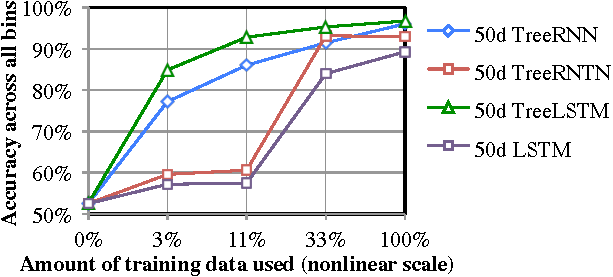
\includegraphics[height=1.1in]{lcc.pdf}
  \caption{Learning curve for the $\le6$ experiment.}
  \label{fig:lc} 
\end{figure}

\section{Results and discussion}\label{sec:discussion}

The results are shown in Figure~\ref{prop-results}. All four models were able to largely memorize the training data (??.?, ??.?, ??.?, and ??.? across bins for the $\le$6 setting, for example). In the $\le$6 setting, the three tree models were able to perform at above ??\% on examples of size $\le$2 with a steady decay in performance continuing through ??.?\% at size 12, and similar, if steeper, decays with smaller training sets. All four robustly beat the simple baselines reported in Bowman et al.: the most frequent class occurs just over 50\% of the time, and a summing model that ignores word order does reasonably on the shortest examples but falls below 60\% by bin 4.

The LSTM performs fairly poorly in the $\le3$ setting, with performance at 3 a mediocre ??.?\%, and an abrupt drop to \% at 4, suggesting that the model did not acquire the needed generalizations. With more ample training data in the $\le6$ condition, though, the LSTM shows fairly good accuracy on short examples, and a smooth decay with no abrupt drop. 

The learning curve (Figure~\ref{fig:lc}) suggests that additional data is unlikely to change these basic results, though the disparity in performance at the 11\% level is striking: the LSTM sequence model and the TreeRNTN (the model with the most parameters by far) lag far behind the other two.

\section{Conclusion}

We find that all four models can exploit recursive structure to interpret sentences with complex unseen structures, and that tree models' biases allow them to learn to do this more effectively from less data. 
We interpret these results as evidence that the similar performance of tree and sequence models can be attributed to their fundamentally similar representational systems, with both models recognizing compositional structure when it is present, the former doing so more reliably, and the latter benefiting elsewhere---either because of architectural choices that make backpropagation more effective, or because interpreting sentences from left to right allows the model to better simulate other aspects of human language comprehension. We finally suggest that, because of the well supported linguistic claim that the kind of recursive structure that we study here is key to language understanding, there is likely to be value in developing sequence models that can more efficiently exploit this structure without fully sacrificing the flexibility that makes these models succeed.
